\section{Patrick Höfner}
\textbf{Responsibility: Back-End, Android-Development}\\
\textbf{Role: Wiki Master}\\

\subsection{Webserver}

To store the information collected via smartphone, a central storage location was required where the data could be stored persistently and made available to all communication partners. One central advantage of our system is to provide data-sovereignty on the patient side. This means that every health-care provider should be able to host a standalone system within his institution to guarantee that the collected patient-data can only accessed by a limited amount of trusted people.This trusted group has to be defined by the patient itself. The simplest and most cost-effective hardware to implement this project was a Raspberry Pi Model 3, which was provided by the university.
The Pi offered the necessary performance to process the data traffic and to host a web application. On the software side, the Raspberry Pi was installed with the operating system Raspbian\footnote{https://www.raspberrypi.org/downloads/raspbian/} in version 10 \glqq{}buster\grqq{}. This is a Linux distribution specially developed for the Pi and makes the best possible use of the limited hardware. A database management system was required to store, manage and process information. MariaDB\footnote{https://mariadb.org/} was chosen for this purpose. This provides a good compromise between performance and database features, such as security functions. In addition, the use of this software solution is classified as \glqq{}open-source\grqq{}, widely used and well documented, which was the most important selection criterion for rapid project progress.

To simplify database administration, PHPMyAdmin\footnote{https://www.phpmyadmin.net/} was installed, which provides a simple local web interface for database administration. Furthermore, an Apache web-server was installed, which will be used in the long run to access the website and database interface (API) via a browser. To realize such an interface a backend was needed which processes all database requests of the web and Android application and performs the necessary operations on the database. For this purpose the Django framework was chosen. This framework integrates important features like an authentication system with users and roles, security features as well as predefined libraries for the creation of database interfaces. The physical web server was installed on a Fritzbox 7530 in the apartment of a team member. 

However, there were some challenges to make the server accessible via the Internet. After several failed attempts, it turned out that most providers only assign IPv6 addresses, which led to accessibility problems. Thus the server was only accessible via devices which assigned an IPv6 address themselves. After a long search for a solution, this issue could be solved at least temporarily via a free service. The service named "ngrok"\footnote{https://ngrok.com/} provides a secure tunnel and a domain to make local web servers accessible via the Internet. Under the provided URL the server could be reached by all devices. However, this is not an appropriate solution in the long run, since the use of this external service should only be used for test purposes. This means the application should be accessible via the Apache web-server over a structured and well understandable domain. Moreover there should be installed dedicated security certificates for our web-service.


\subsection{Database Schema}
A database schema was designed to store the data in the database in a structured manner and to ensure that the integrity of the stored data is guaranteed. Due to the complexity of the application context, a number of database objects had to be considered. The basic concept of the database design is based on the assumption that all database objects can be uniquely assigned to one user. This database design originates from the authentication concept of the Django framework. There a so-called "user-model" is implemented, which can be assigned different roles and rights. Roles would be patients, doctors and relatives in the concrete use case. 


\begin{figure}[h]
    \centering
    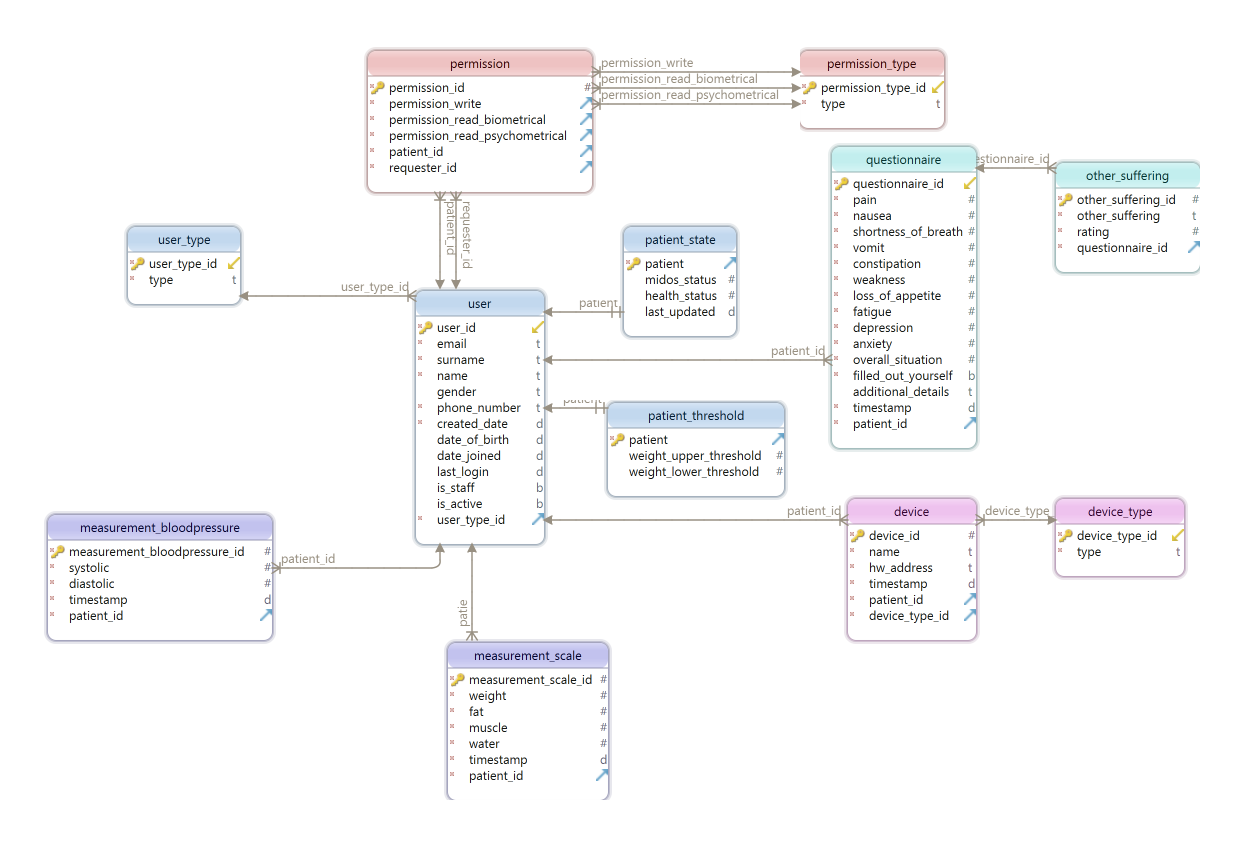
\includegraphics[width = \textwidth]{figures/dataScheme_Bericht.png}
    \caption[Database schema]{Database schema}
    \label{fig:DBSchema}
\end{figure}

However, a semantic problem arose when using this approach, since doctors and relatives do not create their own data records for measurements or completed questionnaires, but only access existing data records of specific patients. This problem was solved with an additional table "Permission", which determines which "user" is authorized to access the data of another "user". The "Permission" table also determines the depth of authorization. Additionally there are tables for "patient-state" and "patient-threshold". Therefore the state of a patient gets calculated and stored in the database depending on the thresholds which are set individually for each patient by the doctor. The database schema was created with the software "DBSchema"\footnote{https://dbschema.com/}, which made it possible to display the schema graphically, which was especially advantageous for the communication within the project team (see Figure \ref{fig:DBSchema}). In addition, the schema could be exported as ".sql" file and directly uploaded to the server as database via the PHPMyAdmin interface. Moreover the database was normalized into third normal form. This was important to avoid duplicates and to provide referential integrity. This means for instance, that only user types can be assigned to a user which have been predefined within the user-type table.


In the next step the database was connected to the Django backend. The Django framework is based on the Python programming language, which means that all operations to be performed on the database objects are also programmed in Python. This offers an enormous advantage from the developer's point of view, since no individual SQL statements have to be programmed. Conversely, however, this means that the tables of the MariaDB database must first be translated into Python objects so that the database entries can be accessed via Python code. Django uses a so-called \glqq{}Object-Relational-Mapper\grqq{} to translate existing SQL databases into Python objects, called "models"\footnote{https://docs.djangoproject.com/en/3.0/topics/db/models/}, which represent database tables. Once the database is migrated, the Django framework translates the Python commands into SQL and performs the desired operations on the database. 

\subsection{Visualization of biometric and psychometric information}
The visualization of the measured values for the user was realized by a series of activities, which all have the same basic structure. In defining a uniform structure, the focus was primarily on a simple, clear and comprehensible way of displaying the most important information to a patient without detours. When considering which information is most meaningful for the patient, after discussion and taking user feedback into account, the conclusion was reached that a temporal course of the measured values as well as an average value over a certain time is most informative for the patient. Therefore a basic layout was created for each activity, which implements a tab layout at the top of the screen. This enables the patient to display a time history over a week, a month or a year. The values are displayed using different types of graphs, which are adapted to the information displayed, and implement a red line for a maximum value that can be defined by a doctor in advance (see Figure \ref{fig:Screenshot1} a,b; \ref{fig:Screenshot2} b).

\begin{figure}[ht]
    \centering
    \subfigure[Weight activity]{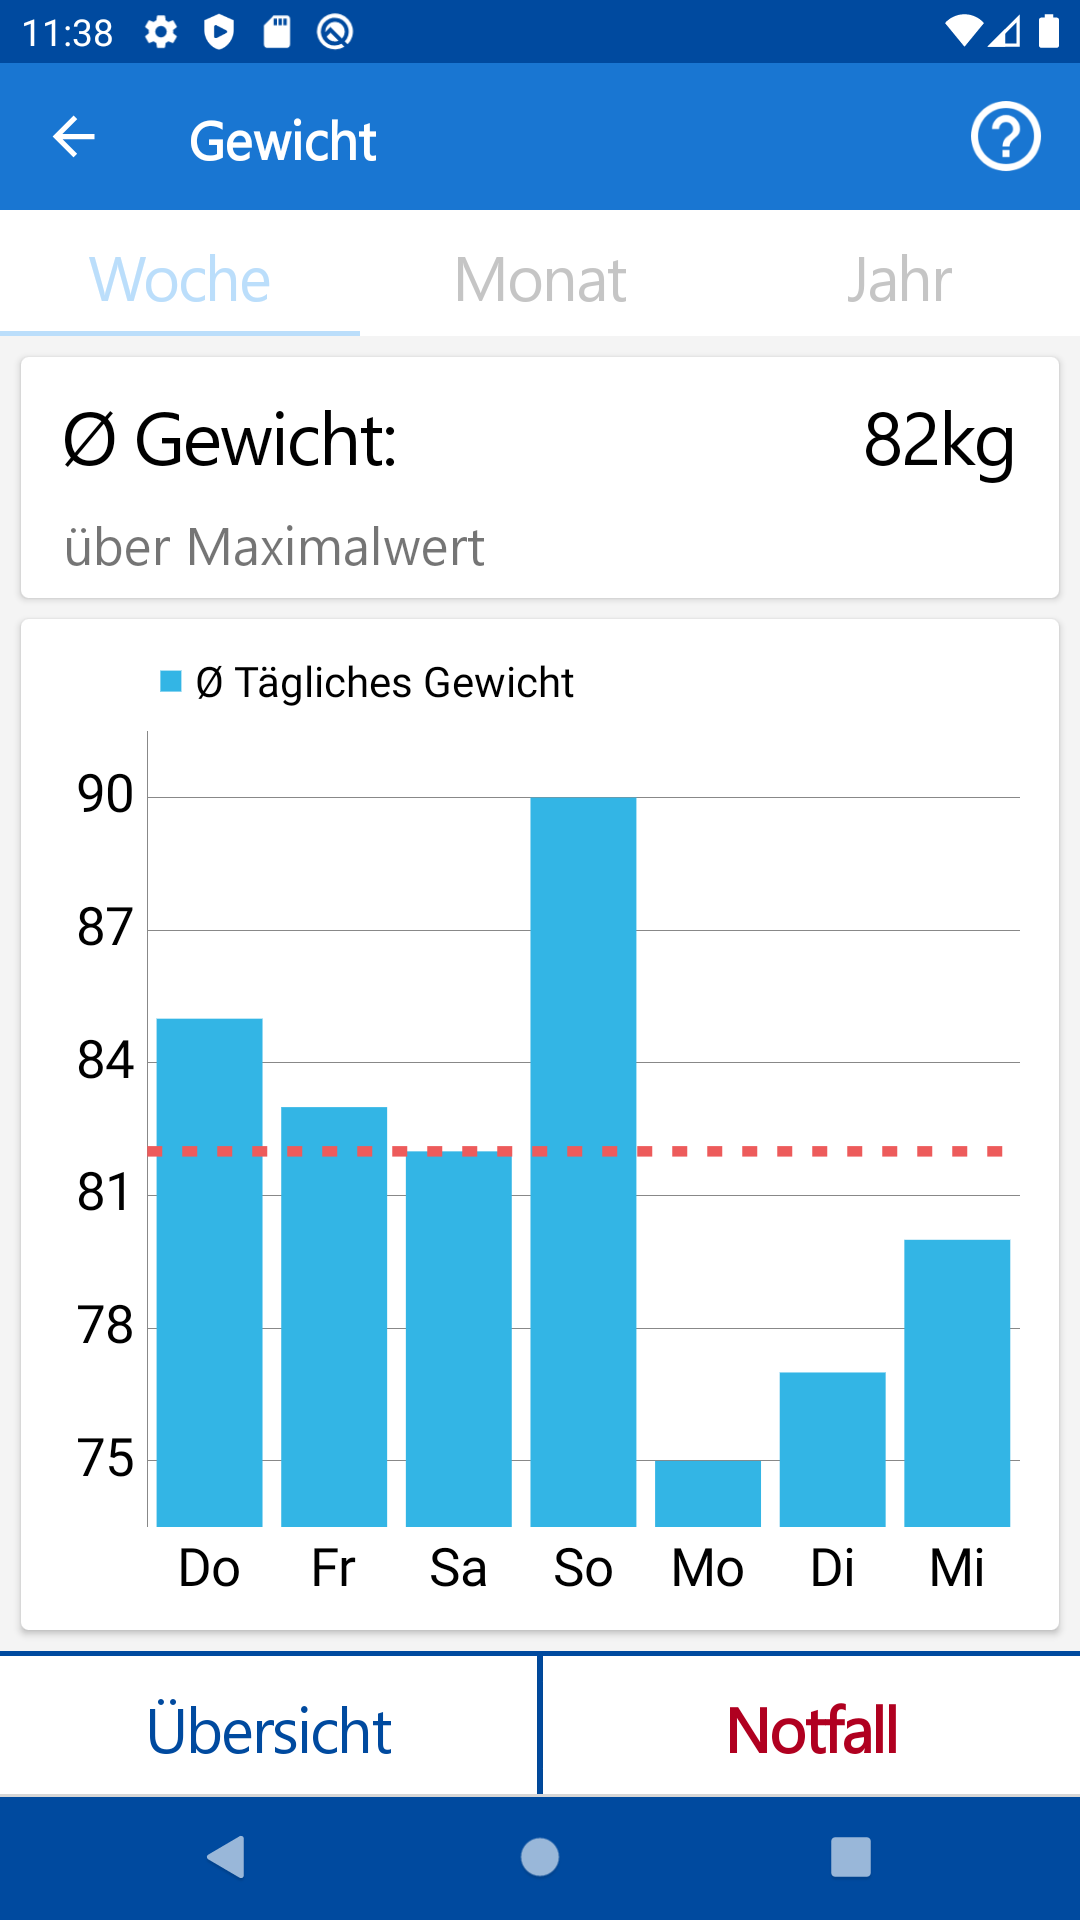
\includegraphics[width=0.30\textwidth]{figures/Screenshot_1584112496.png}}
    \subfigure[Bloodpressure activity]{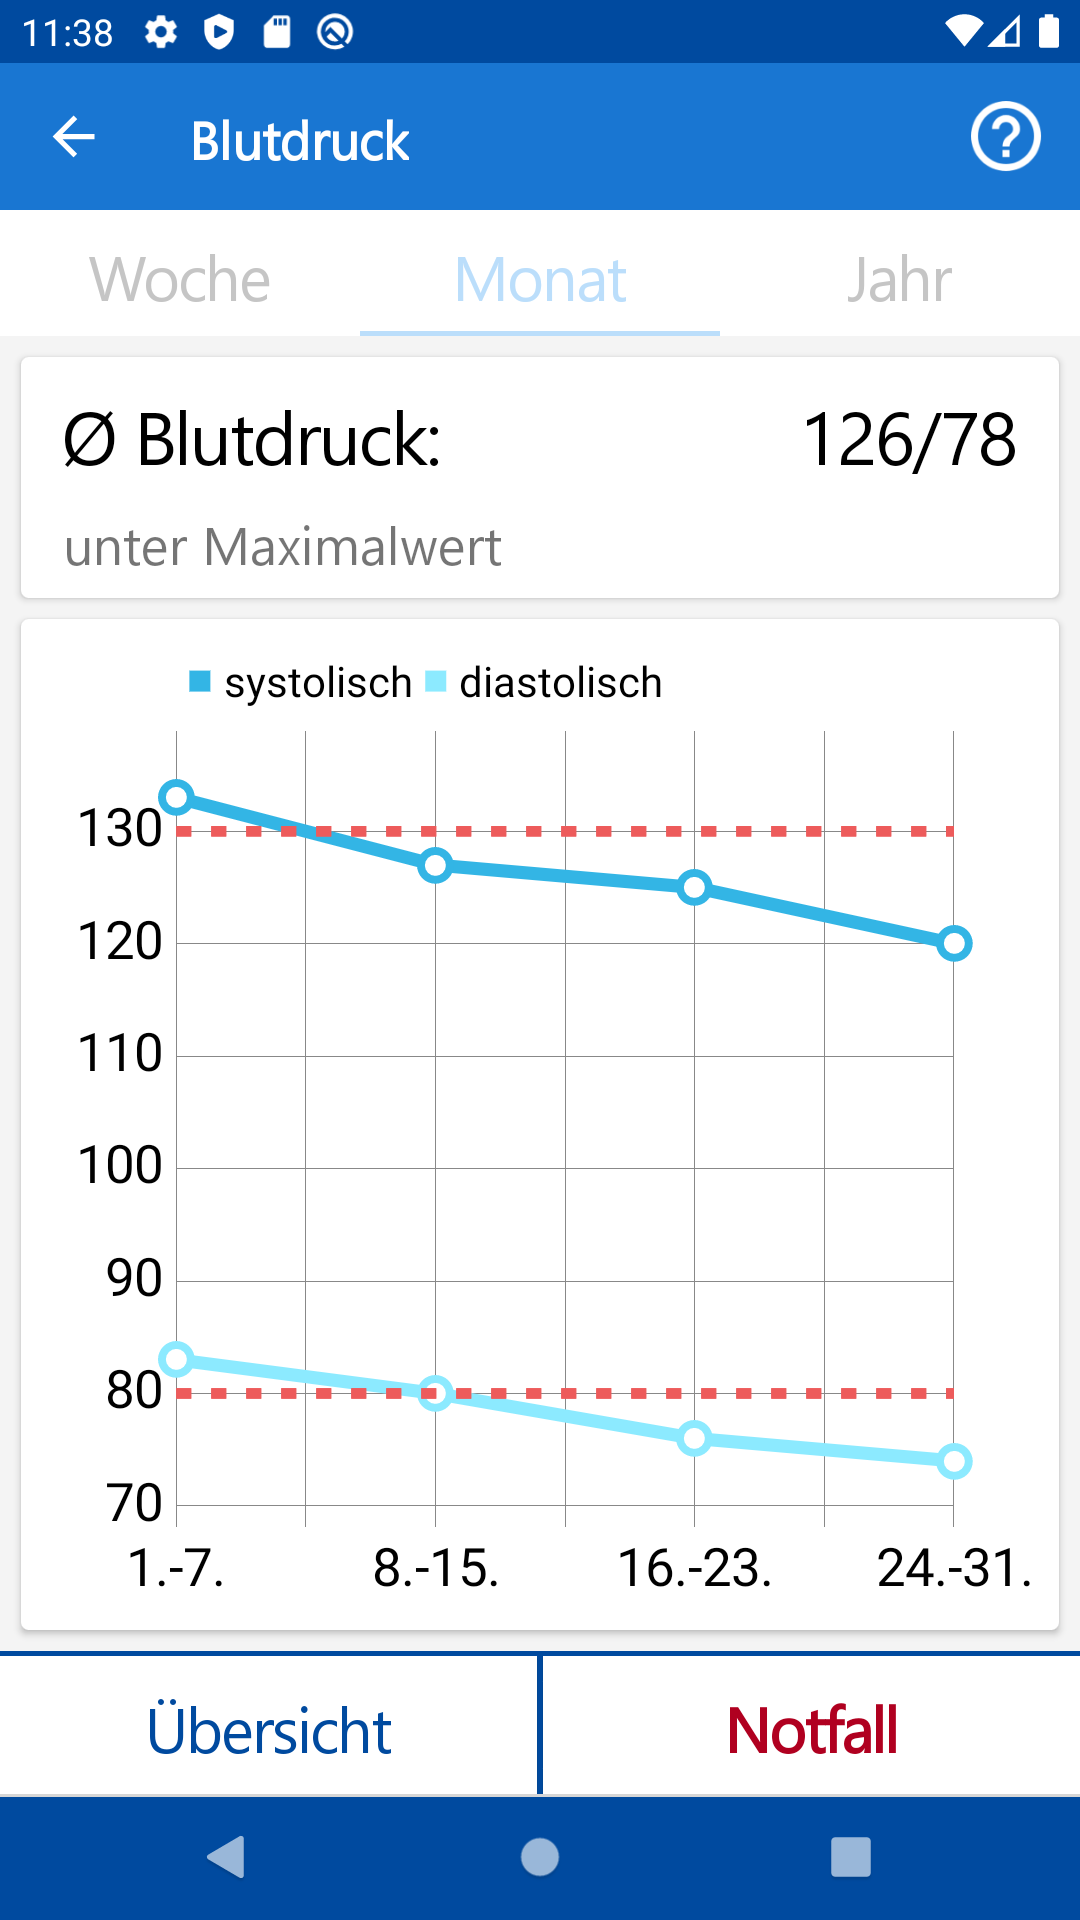
\includegraphics[width=0.30\textwidth]{figures/Screenshot_1584112512.png}}
    \caption[Screenshots of activities displaying biometrical information to the user]{\tabular[t]{@{}l@{}}Screenshots of activities displaying biometrical information to the user \endtabular}
    \label{fig:Screenshot1}
\end{figure}

The library \glqq{}MPAndroidChart\grqq{}\footnote{https://github.com/PhilJay/MPAndroidChart} was used to display graphs in the Android application. This library provides a number of very flexible customizable graphs and offers a good overall package due to its variety and good documentation. After the github repository was integrated into the Android project, all available functions of this library could be used. All values and value limits of the x- and y-axis are freely customizable which allows to display qualitative values. First of all, the display of biometric values - blood pressure and weight - was taken into account during the development, since the first development steps focused on the recording of data via the scales. For the display of weight we decided to use a bar chart because of the easy interpretation of quantitative values and the good recognizability of a time sequence (see Figure \ref{fig:Screenshot1} a). In order to display blood pressure, two related values are needed, the systolic and diastolic values. Therefore a line chart was used to display the blood pressure (see Figure \ref{fig:Screenshot1} b). Since the two values always have a distance between them, overlapping of the lines is impossible. Furthermore, the arrangement of the two related values on top of each other and auxiliary lines in the graph make it possible for the user to recognize relations.

\begin{figure}[h!]
    \centering
    \subfigure[Sufferings overview]{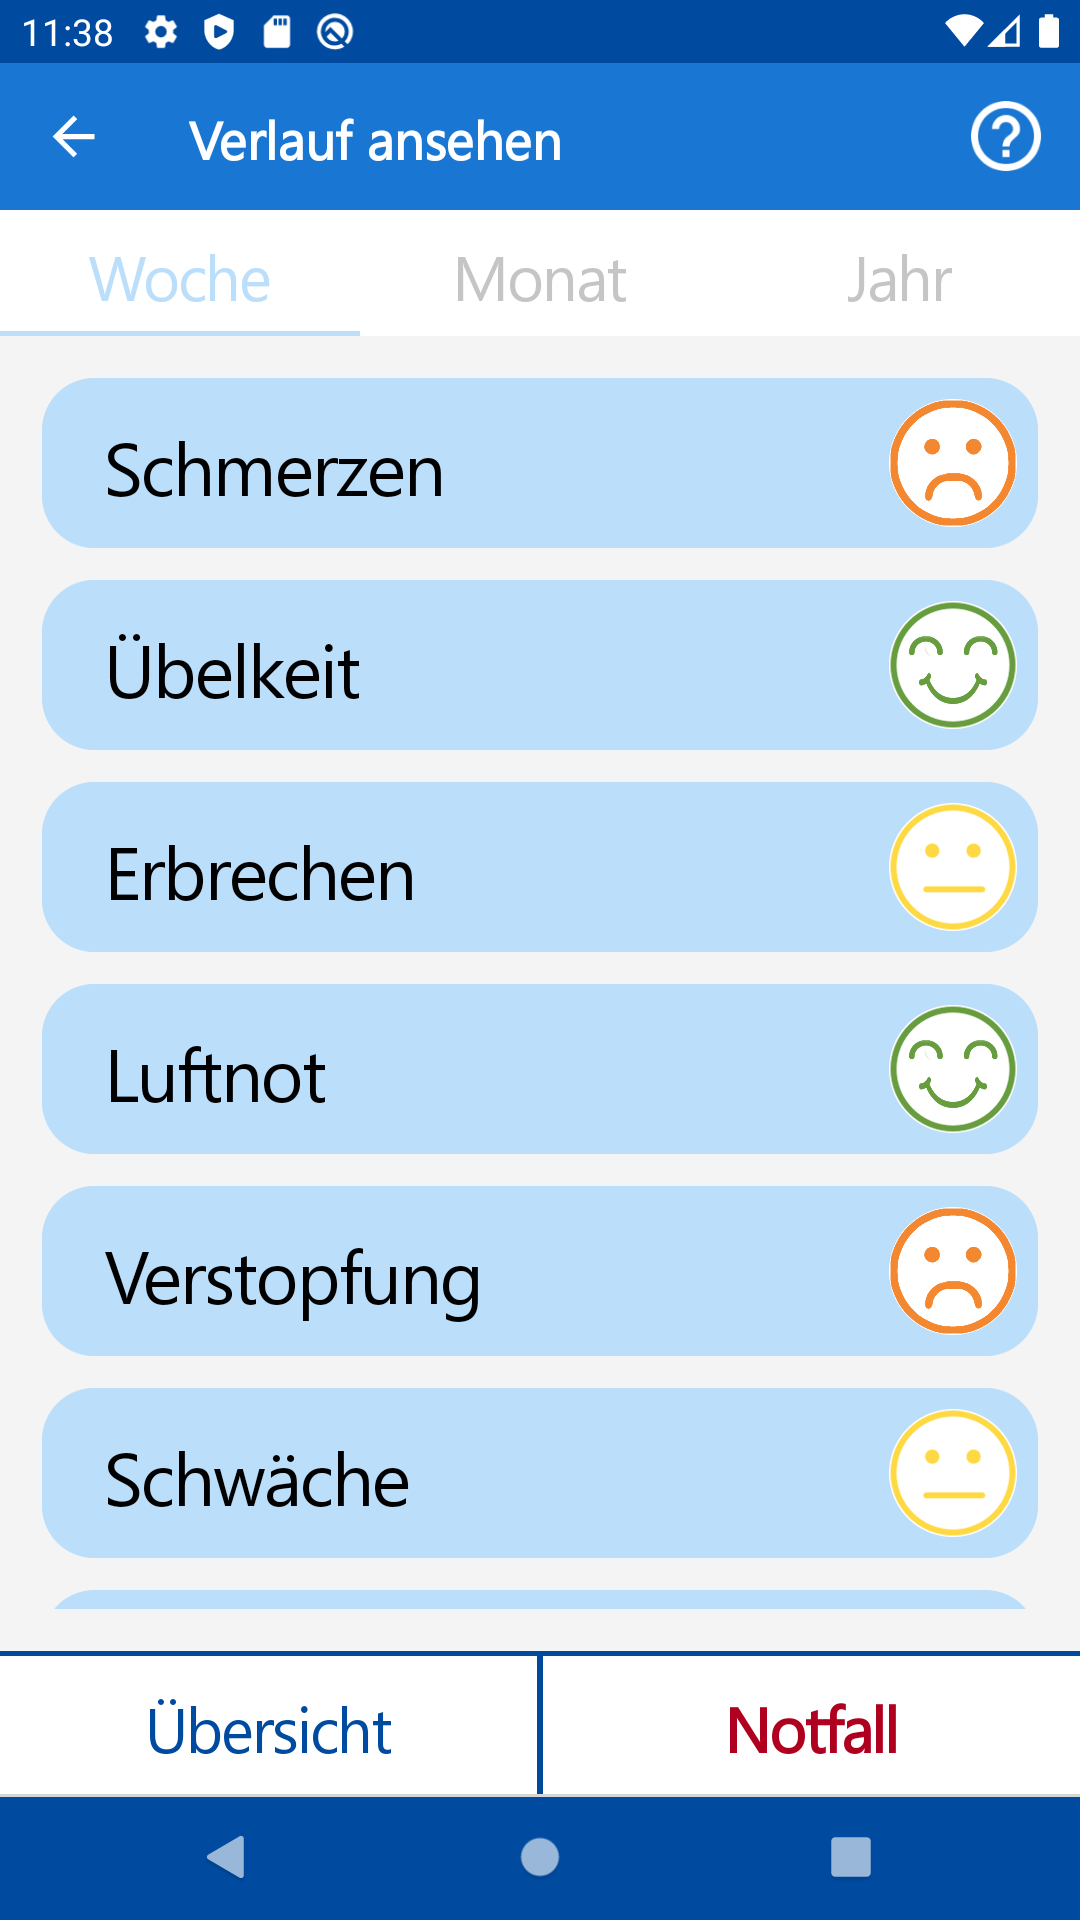
\includegraphics[width=0.30\textwidth]{figures/Screenshot_1584112527.png}}
    \subfigure[Sufferings detailed view]{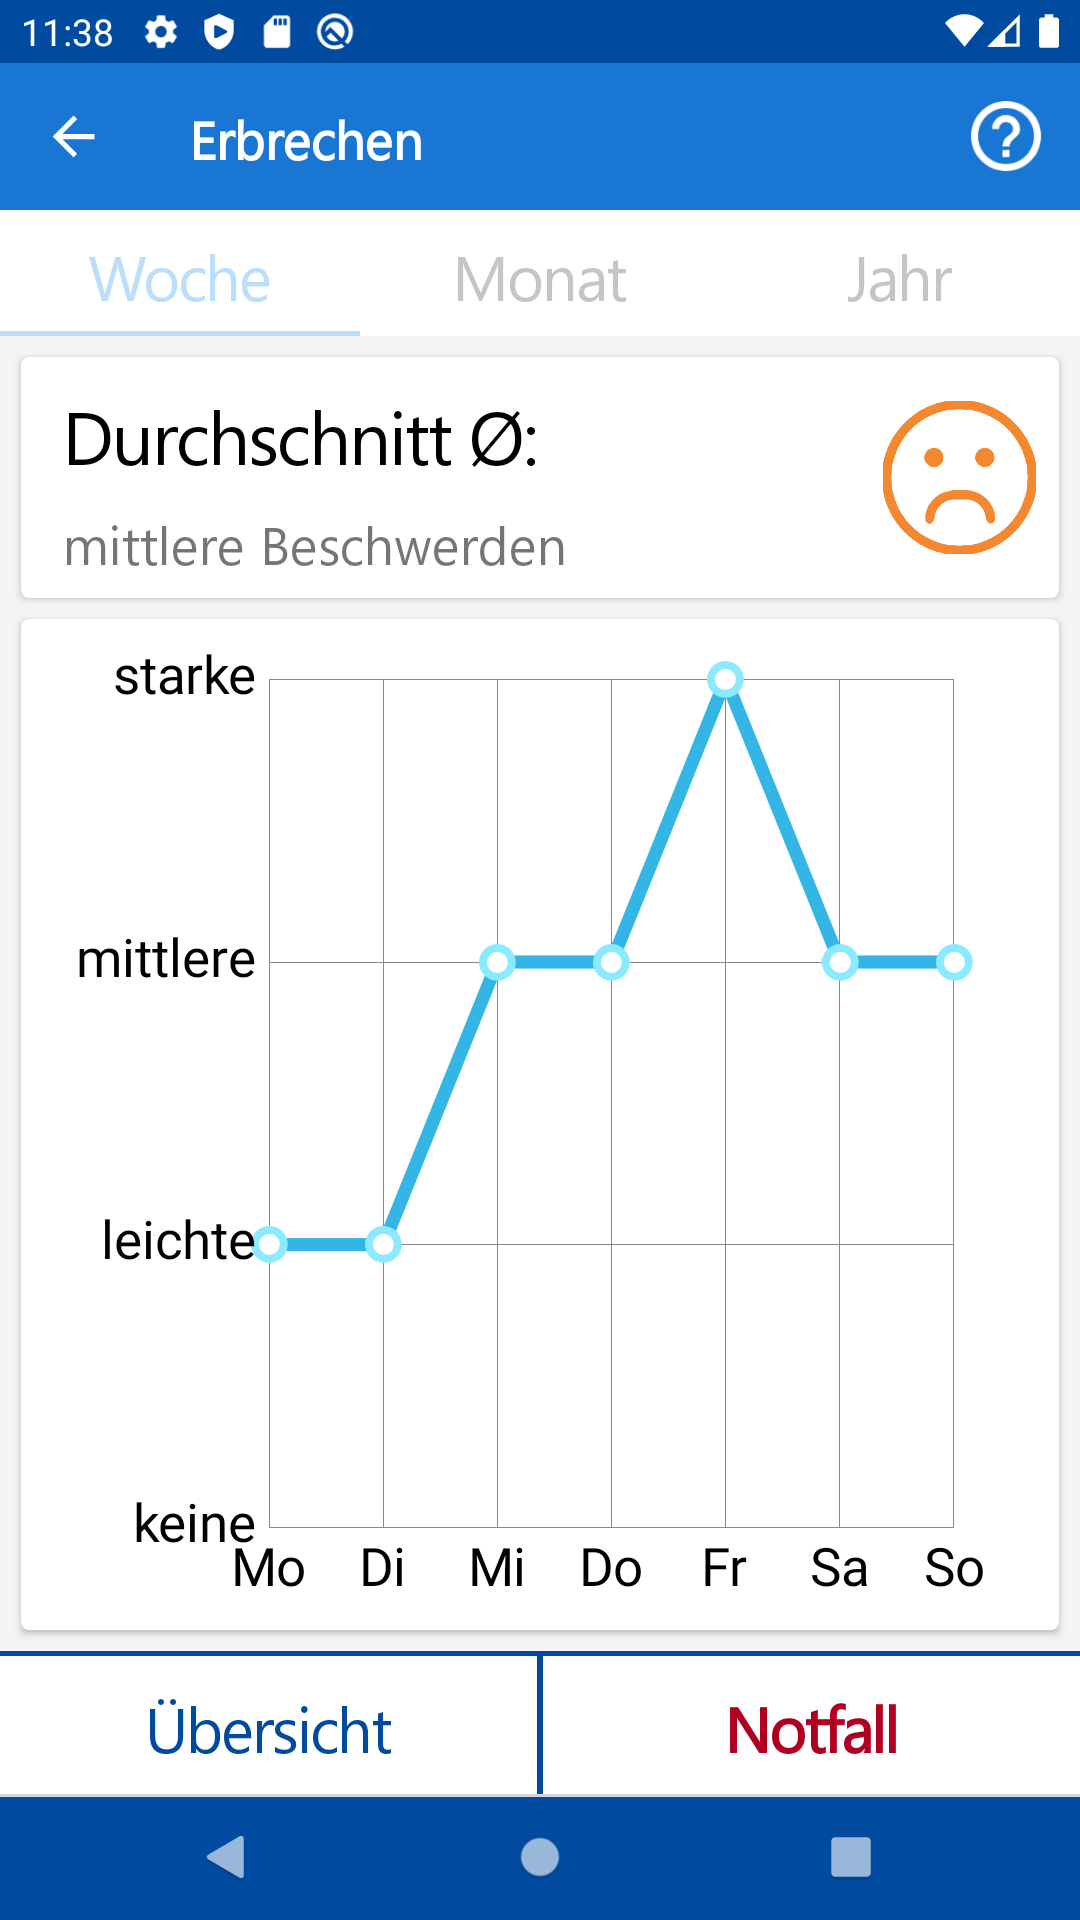
\includegraphics[width=0.30\textwidth]{figures/Screenshot_1584112570.png}}
    \caption[Screenshots of activities displaying psychometric information to the user]{\tabular[t]{@{}l@{}}Screenshots of activities displaying psychometric information to the user \endtabular}
    \label{fig:Screenshot2}
\end{figure}

Since problems with clarity arose when displaying all days of a calendar month or all months of a year due to the limited screen size, certain periods were combined. This means, for example, that in the year view an average value for the months January to March is shown in the graph and the individual months are not shown broken down for themselves (see Figure \ref{fig:Screenshot1} b). When implementing a view for the psychometric data, an additional overview activity was integrated, which provides an overview of all the conditions recorded in the questionnaire. Here the patient can see at first glance whether the recorded complaints were non-existent, mild, moderate or severe. Also in this view a certain period of time can be selected for the view via the Tab-layout (see Figure \ref{fig:Screenshot2} a). If a patient would like to get more detailed information about a certain ailment, he can click on the respective button to get to the detailed view. There, analogous to the biometric information, a line chart is displayed, whereby a line chart was chosen based on the qualitative values (see Figure \ref{fig:Screenshot2} b). 

\subsection{REST-API}
Django REST framework\footnote{https://www.django-rest-framework.org/} was used to store and retrieve data on the server via the internet. It can be seamlessly integrated into Django and provides the most important functions for defining an Application Programming Interface (API). API defines a set of endpoints that can be used to perform certain operations on the server's database by using backend functionality. Each endpoint is assigned its own domain, through which certain information can be retrieved or stored. Within the project, so-called GET and POST requests were used, which are sent from the client to the server.  This could be managed by implementing the libary "Retrofit"\footnote{https://square.github.io/retrofit/} within the Android application which will be explained in further detail later on. With a GET-request data can be retrieved from the server and with a POST-request a new data set can be created on the server. The JSON\footnote{https://www.json.org/json-en.html} data format is used to transfer data records structured in text form and to interpret them correctly afterwards (see Figure \ref{fig:ClientServer}). 

To ensure successful communication between Android application, server and web application, endpoints for the registration of a new user and the login/logout of an existing user were defined. The Django framework provides predefined functionality to generate a token after successful registration or login, which is needed to retrieve or store data from the server.
The token authentication ensures that only authorized, i.e. registered and logged in users, have access to the data. Due to the individual adaptations of the standard Django user model, a number of adjustments were also necessary when using the given functionality of the Django-REST-Famework. Besides registration and login endpoints, there were defined endpoints to access data about users, patient-status and questionnaires.

\begin{figure}[h]
    \centering
    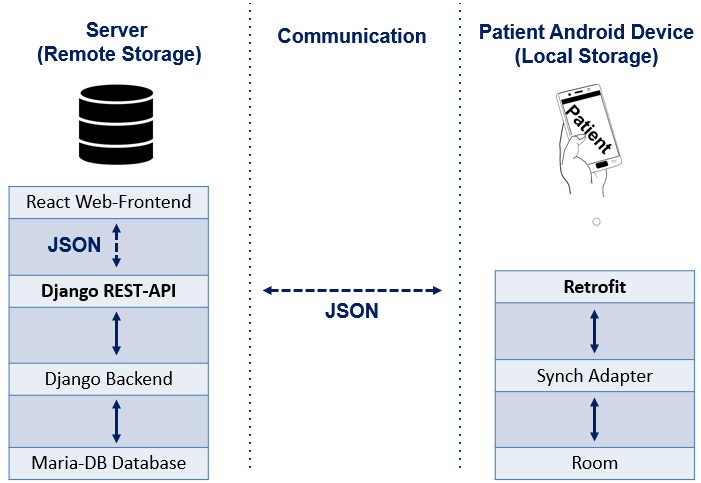
\includegraphics[width = \textwidth]{figures/Client-Server-Architecture.png}
    \caption[Database schema]{Description of the client-server-architecture}
    \label{fig:ClientServer}
\end{figure}